\section{Исследование и построение решения задачи}
\label{sec:Chapter3} \index{Chapter3}

Согласно главе~\ref{sec:Chapter2}, наилучшие результаты в решении задачи распознавания рукописного текста себя показывают
модели с архитектурой seq2seq и, в частности, трансформеры.
В рамках данной задачи, одним из самых значительных препятствий на пути её решения является недостаток данных,
требуемых для обучения вышеописанных моделей.
В силу трудоёмкости процесса создания большого размеченного набора данных рукописных текстов, применяются техники генерации синтетических данных.
На данный момент предложено несколько подобных техник (см. секцию~\ref{subsubsec:generation}).
Два наиболее известных способа -- это использование рукописных шрифтов и генеративно-состязательных сетей.
Сравнение эффективности использования синтетических данных, сгенерированных различными способами, может позволить понять,
что стоит использовать для получения наилучших результатов.
При этом желательно провести исследование на моделях различных архитектур для того, чтобы избежать
подстраивания экспериментов под особенности конкретной архитектуры.
На текущий момент времени, в существующих научных работах подобного исследования описано не было, насколько это может быть известно.

Если рассматривать задачу распознавания рукописного текста на русском языке,
то здесь сравнение методов расширения наборов данных также является актуальным в силу недостатка научных работ в этой области.
Единственным примером для русского языка служит работа~\cite{shonenkov2021stackmix},
в которой алгоритм генерации полу-синтетических данных Stackmix позволил повысить точность распознавания модели с 71\% до 80\% на наборе HKR.
В дополнение к этому, в научной литературе не упоминается использование самого популярного метода создания синтетических данных
на основе рукописных шрифтов в контексте русского языка.
Реализация подобного метода требует дополнительных исследований.

Таким образом, предлагается рассмотреть некоторые методы генерации синтетических наборов данных и сравнить их в контексте
задачи распознавания рукописного текста на русском языке:
\begin{itemize}
    \item Генерация изображений текста с помощью рукописных шрифтов;
    \item Алгоритм Stackmix для генерации полу-синтетических изображений~\cite{shonenkov2021stackmix};
    \item Генерация изображений рукописного текста при помощи генеративно-состязательных сетей.
\end{itemize}

При этом предлагается рассмотреть две архитектуры нейронных сетей для тестирования методов:
\begin{itemize}
    \item Seq2seq архитектура~\cite{sutskever2014sequence}, состоящая из сверточной и рекуррентных нейронных сетей с механизмом внимания;
    \item Архитектура трансформер~\cite{vaswani2017attention}.
\end{itemize}

Согласно информации из секции~\ref{subsec:datasets}, для русского языка существует два общедоступных эталонных набора данных,
на которых можно проводить исследования.
Они обладают определёнными особенностями и достаточно сильно отличаются друг от друга,
что позволяет более детально проанализировать эффективность методов расширения наборов данных.


\subsection{Генерация изображений текста с помощью рукописных шрифтов}
\label{subsec:synthetic}

Генерация изображений текста с помощью рукописных шрифтов -- наиболее простой способ создания дополнительного обучающего набора данных.
Этот метод не требует обучения дополнительных моделей, не зависит от какого-либо фиксированного набора данных,
прост в реализации и позволяет генерировать данные с большой скоростью.
Несмотря на многочисленные достоинства, генерация текста с помощью шрифтов обладает рядом недостатков.
Типографские шрифты, даже рукописные, не обладают достаточным разнообразием и выглядят искусственно не только для нейронной сети,
но и для человеческого глаза.
Как правило, в шрифтах содержится ограниченное количество доступных для написания символов, что влечет за собой зависимость метода от
того языка, для которого генерируются дополнительные данные.

Ещё одним существенным недостатком является сложность добавления нового стиля написания, т.е. непосредственно шрифта,
так как, как правило, для этого необходимо большое количество времени и умение работать со специализированным программным обеспечением.
Этот недостаток сильно заметен по отношению к кириллическим шрифтам -- существует не так много открытых рукописных шрифтов, содержащих русские символы.
Поэтому имеет смысл каким-то образом автоматизировать процесс создания нового шрифта.
В этом может помочь приложение \textit{calligraphr}\footnote{\url{https://www.calligraphr.com}},
позволяющее из изображений символов получить шрифт в формате \textit{ttf}.
Изображения рукописных символов можно взять из базы символов, описанной в секции~\ref{subsec:datasets},
в которой для каждого рукописного кириллического символа существует более 1500 вариантов написания.

Приложение \textit{calligraphr} требует заполнения шаблона с заранее выбранным набором символов.
Шаблон представляет собой изображение, содержащее таблицу, в которой в определённых ячейках должны помещаться изображения конкретных символов.
Пример пустого и заполненного шаблона представлен на рисунке~\ref{fig:templates}.

\begin{figure}[h!]
    \centering
    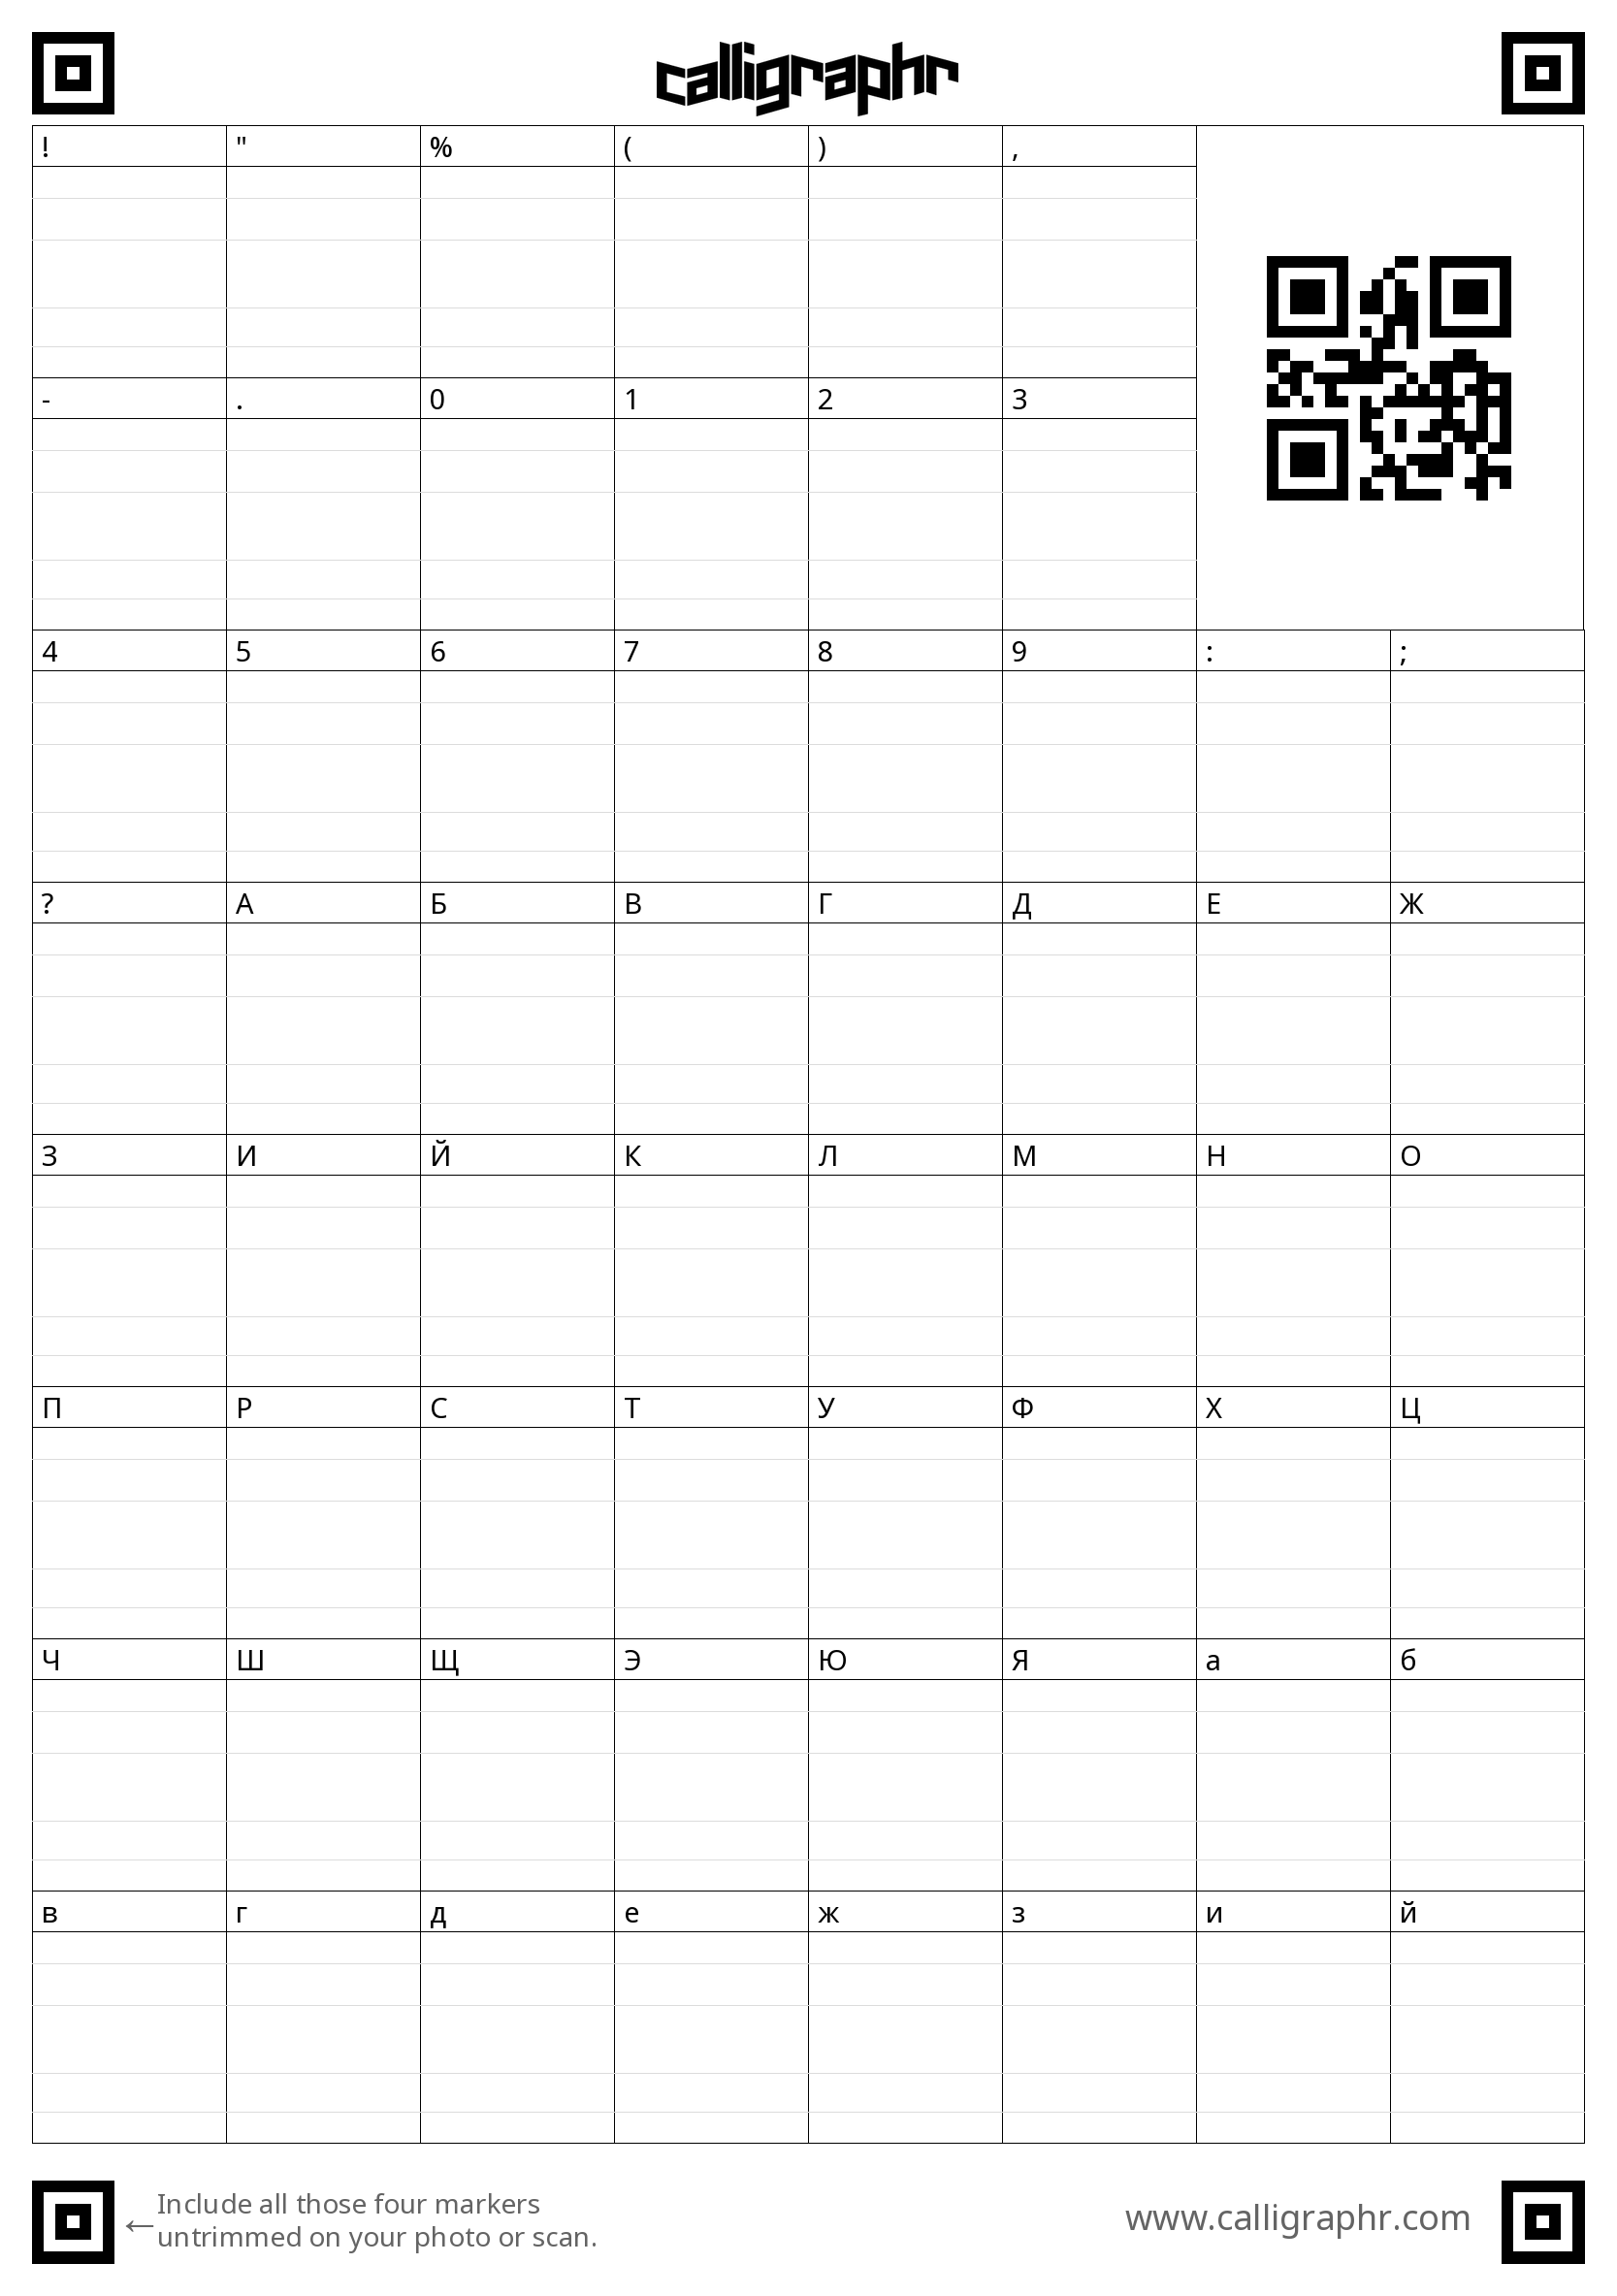
\includegraphics[width=0.45\textwidth]{img/template}
    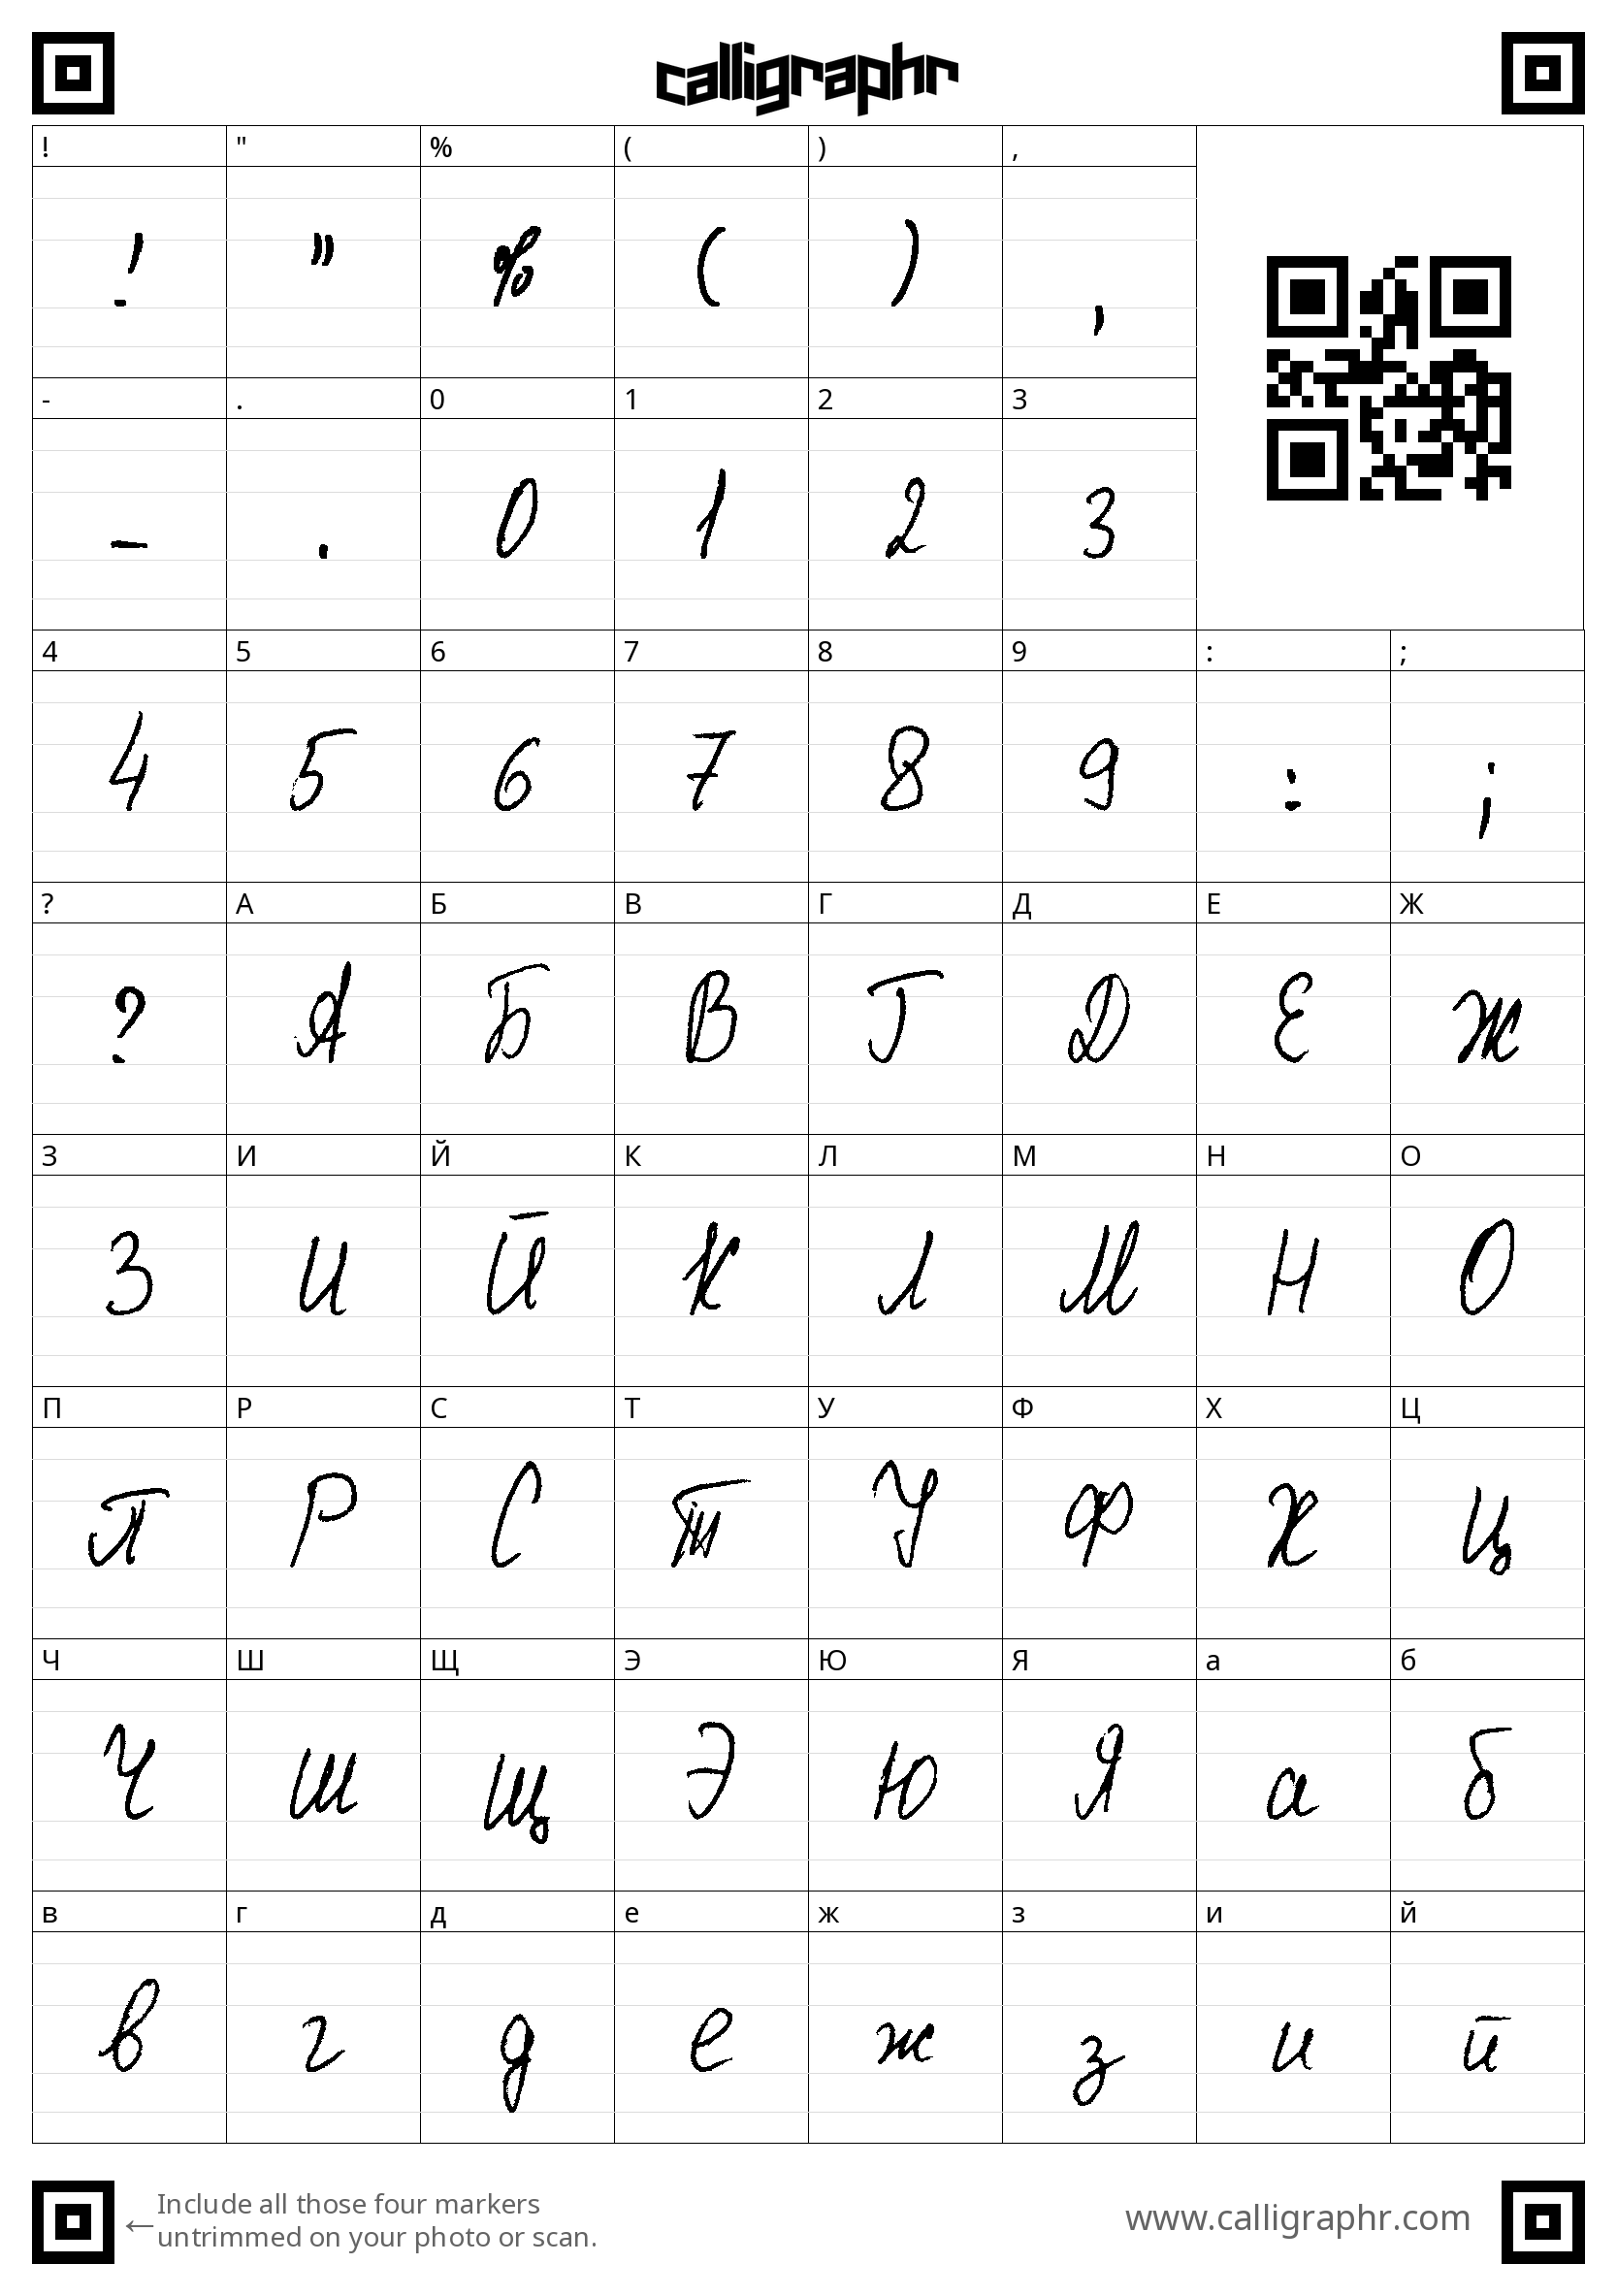
\includegraphics[width=0.45\textwidth]{img/template_filled}
    \caption{Примеры пустого и заполненного шаблонов для приложения \textit{calligraphr}}
    \label{fig:templates}
\end{figure}

Заполненный шаблон далее анализируется приложением, которое извлекает глифы -- векторные изображения символов.
У полученных глифов можно вручную поменять расположение и размер, таким образом прибавив реалистичности к результату.
Затем из глифов формируется шрифт необходимого формата.
Таким образом, создание шрифта можно определенным образом автоматизировать.

Для создания нового кириллического шрифта предлагается следующая последовательность действий:
\begin{enumerate}
    \item Заполнение шаблона для \textit{calligraphr} изображениями кириллических символов;
    \item Ручная коррекция полученных с помощью \textit{calligraphr} глифов при необходимости;
    \item Итоговая сборка шрифта.
\end{enumerate}

Последние два пункта алгоритма выполняются непосредственно с помощью приложения.
Первый пункт требует анализа границ шаблона для поиска координат вставки изображений,
а также нахождения базовой линии символа для того, чтобы вставить его в соответствии с ней.
Границы шаблона можно найти с помощью комбинации морфологических операций \textit{dilate} и \textit{erode},
например, как это сделано для анализа таблиц в библиотеке \textit{dedoc}\footnote{\url{https://github.com/ispras/dedoc}}.
Эти границы можно найти один раз и зафиксировать для конкретного шаблона.
Нахождение базовой линии символа можно с некоторыми оговорками реализовать аналогично нахождению базовой линии слова,
для этого существует метод на основе устойчивой регрессии, описанный в работе~\cite{sueiras2021continuous}.
В силу того, что для символов базовую линию находить сложнее, требуется дополнительная коррекция на втором шаге алгоритма.

Пример одного из шрифтов, полученных с помощью описанного выше алгоритма, представлен на рисунке~\ref{fig:font_example}.

\begin{figure}[h!]
    \centering
    \frame{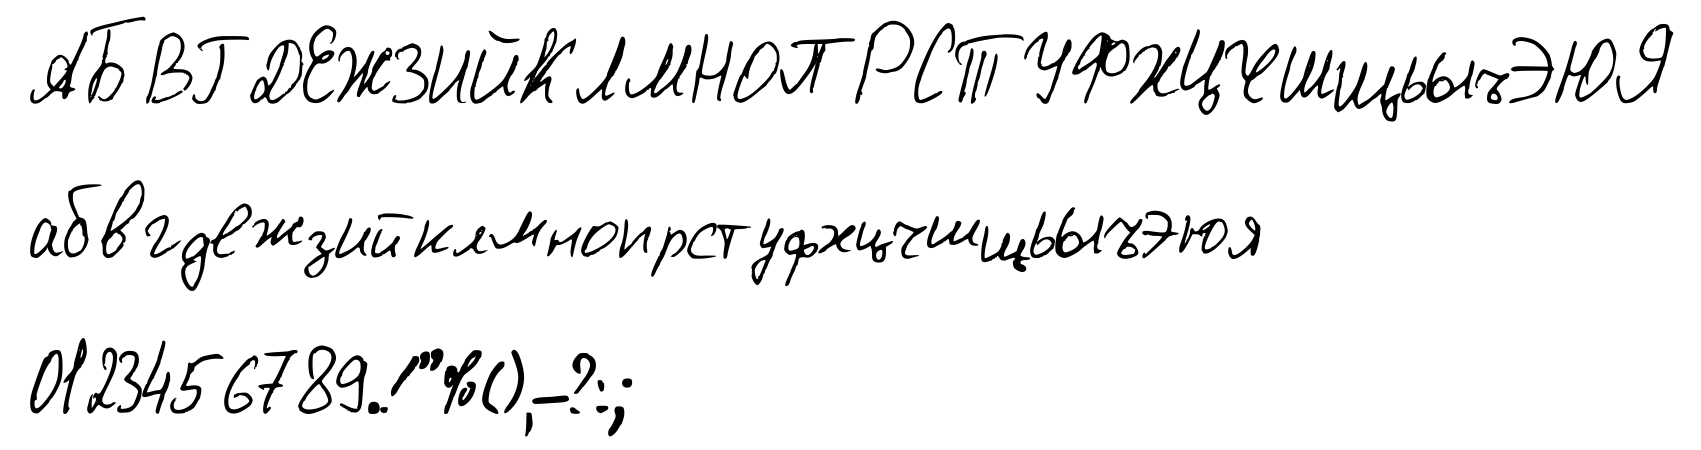
\includegraphics[width=0.8\textwidth]{img/font_example}}
    \caption{Пример шрифта, сгенерированного с помощью приложения \textit{calligraphr} и базы символов}
    \label{fig:font_example}
\end{figure}

Помимо создания новых шрифтов, можно использовать немногочисленные доступные кириллические рукописные шрифты.
При наличии нескольких десятков шрифтов можно реализовать генератор рукописного текста с помощью многочисленных библиотек
отрисовки текста на изображении, и далее создавать достаточно разнообразные синтетические изображения рукописного текста.
Более того, к имеющимся возможностям можно добавить некоторую рандомизацию, напоминающую аугментацию изображений.
При создании изображений можно использовать следующие аугментации:
\begin{itemize}
    \item Изменение размера шрифта, сжатие изображения;
    \item Шумы различных видов (Гауссовский, ISO, мультипликативный);
    \item Размытие различных видов (движения, медианное);
    \item Морфологические операции (эрозия, диляция) для изменения толщины символов;
    \item Изменение наклона шрифта согласно алгоритму из работы~\cite{sueiras2021continuous};
    \item Искажение перспективы изображения;
    \item Небольшие обрезка и повороты изображения;
    \item Имитация рукописных зачеркиваний, описанная в работе~\cite{shonenkov2021stackmix};
    \item Вставка обрезанных символов по краям изображения (имитация соседних строк);
    \item Добавление случайных (светлых, темных) пятен на изображение;
    \item Изменение яркости, контрастности, насыщенности изображения.
\end{itemize}

Таким образом, разработан метод генерации изображений рукописного текста на основе кириллических шрифтов.
Примеры результатов работы генератора рукописного текста представлены на рисунке~\ref{fig:synthetic_example}.

\begin{figure}[h!]
    \centering
    \frame{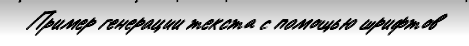
\includegraphics[width=0.9\textwidth]{img/synthetic_cyrillic}}
    \frame{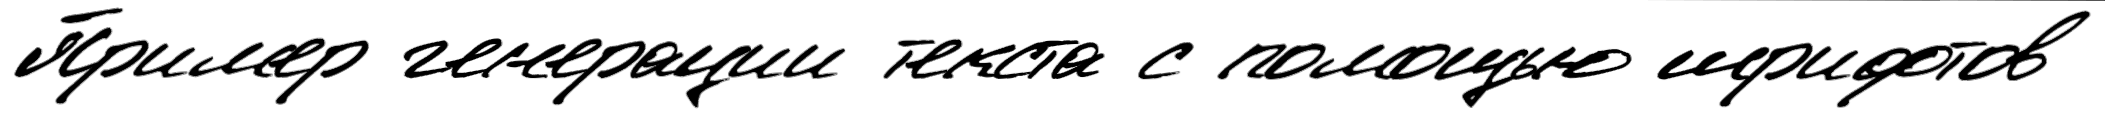
\includegraphics[width=0.9\textwidth]{img/synthetic_hkr}}
    \caption{Примеры результатов работы генератора рукописного текста}
    \label{fig:synthetic_example}
\end{figure}


\subsection{Алгоритм Stackmix для генерации изображений}
\label{subsec:stackmix}

Данный алгоритм генерации синтетических изображений рукописного текста в общих чертах описан в секции~\ref{subsubsec:generation}.
Основной смысл метода заключается в том, что из имеющегося набора данных с фиксированным словарём можно создавать новые слова/предложения
путем нарезки частей имеющих слов и склейки новых слов из этих частей.
Таким образом, метод позволяет модели лучше заточиться под конкретный набор данных, при этом не переобучиваясь на фиксированном наборе слов.
Авторам алгоритма~\cite{shonenkov2021stackmix} удалось существенно поднять качество распознавания предложенной ими модели
на нескольких наборах данных.
Например, благодаря такому расширению наборов, для набора данных HKR точность распознавания увеличилась на 9\%.

Более детально, для того, чтобы использовать метод Stackmix для генерации изображений, нужно выполнить следующую последовательность действий:
\begin{enumerate}
    \item Обучить модель распознавания рукописного текста, предложенную авторами, на обучающем наборе, который планируется расширять;
    \item С помощью обученной на предыдущем шаге модели сгенерировать так называемые символьные маски -- информацию о координатах границ символов в каждом изображении слова из набора данных.
    Эту информацию предоставляет декодер CTC~\cite{graves2006connectionist}, который является частью предложенной модели.
    \item Сформировать упорядоченный набор обрезанных изображений символов и подслов с настраиваемой максимальной длиной.
    Этот набор будет использоваться для сборки новых слов/предложений из имеющихся нарезок.
    \item Непосредственно запустить алгоритм синтезирования новых слов на основе набора обрезанных изображений символов/подслов.
    Он может быть запущен предварительно на фиксированном корпусе слов, либо использоваться для генерации обучающих примеров во время обучения сети.
\end{enumerate}

Как видно из описания метода, у него есть существенный недостаток -- необходимость в обучении дополнительной модели для получения координат границ символов.
Слово нарезается на символы вертикально -- это означает, что для почерков с наклоном части символов будут обрезаны.
При этом сама модель дает предсказания не со 100\%-ной точностью, что также влияет на качество разделения слов на символы.
И, в дополнение к вышеперечисленному, при склейке нет анализа того, на какой высоте находится очередной символ, поэтому соединения
могут получаться слишком неестественными, а слова -- нечитаемыми.

Несмотря на явные минусы, этот метод всё-таки выполняет свою основную функцию -- набор данных увеличивается довольно
нестандартным способом, который может предотвратить переобучение модели.
При этом, большим плюсом является то, что исходный код метода выложен в открытый доступ\footnote{\url{https://github.com/ai-forever/StackMix-OCR}},
что предоставляет возможность провести эксперименты для проверки эффективности метода.

Примеры результатов работы алгоритма Stackmix на наборах данных HKR и Cyrillic Handwriting Dataset представлены на рисунке~\ref{fig:stackmix_example}.
По примерам, представленным на рисунке, можно сделать вывод, что метод в большей степени подходит для наборов изображений с однородным фоном и
относительно одинаковыми условиями написания текста, что характерно для набора HKR и совершенно несвойственно набору Cyrillic Handwriting Dataset.
Тем не менее, можно попытаться сгладить эффект неоднородности путем предобработки изображений, например, с помощью алгоритмов бинаризации (см. секцию~\ref{subsec:preprocessing}).

\begin{figure}[h!]
    \centering
    \frame{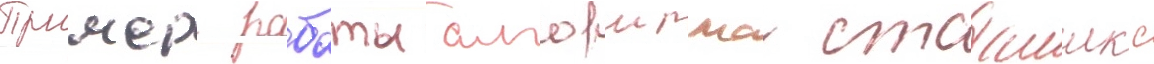
\includegraphics[width=0.9\textwidth]{img/stackmix_hkr}}
    \frame{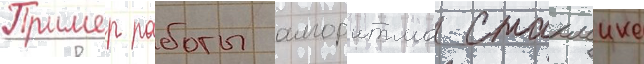
\includegraphics[width=0.9\textwidth]{img/stackmix_cyrillic}}
    \caption{Примеры результатов работы алгоритма Stackmix (сверху для набора HKR, снизу для набора Cyrillic Handwriting Dataset)}
    \label{fig:stackmix_example}
\end{figure}


\subsection{Генерация изображений рукописного текста при помощи\\генеративно-состязательных сетей}
\label{subsec:gan}

Ещё одной популярной областью для исследований в области генерации изображений рукописного текста является применение генеративно-состязательных сетей (GAN).
Согласно описанию секции~\ref{subsubsec:generation}, такие сети в состоят из генеративной модели, создающей примеры,
и дискриминативной модели, отличающей сгенерированные примеры от настоящих.
Здесь, как и в предыдущем описанном методе Stackmix, также есть недостаток оттого, что нужно обучать еще одну модель.
Более того, генеративно-состязательные сети имеют существенно более сложную архитектуру,
вследствие чего требуются значительные ресурсы для их обучения, которые есть далеко не у всех.

Одной из наиболее современных предложенных сетей, генерирующих изображения текста, является ScrabbleGAN~\cite{fogel2020scrabblegan}.
В отличие от остальных известных новейших моделей, ScrabbleGAN имеет относительно несложную структуру и позволяет получать
изображения различных случайных стилей с помощью встроенного вектора шума.
Еще одним существенным достоинством является то, что код модели доступен, причем в разных вариациях,
которые направлены на исправление ошибок и улучшение качества кода.
Следовательно, при наличии достаточных ресурсов для обучения сети, этот метод также воспроизводим.

На рисунке~\ref{fig:gan_example} представлены примеры обученной генеративно-состязательной сети ScrabbleGAN на
наборах данных HKR и Cyrillic Handwriting Dataset.
Как видно из рисунка, изображения получаются достаточно реалистичными, однако некоторые детали соединения символов и фона
дают понять наблюдателю, что данные синтетические.
Аналогично результатам генерации методом Stackmix, изображения для набора данных HKR получаются более удачными по сравнению с
более сложными и вариативными изображениями для Cyrillic Handwriting Dataset.
Стоит также отметить, что в отличие от двух предыдущих описанных методов, генеративно-состязательные сети позволяют
корректно обработать варьирующиеся соединения символов друг с другом.

\begin{figure}[h!]
    \centering
    \frame{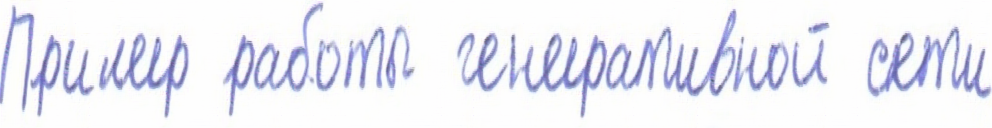
\includegraphics[width=0.9\textwidth]{img/gan_hkr}}
    \frame{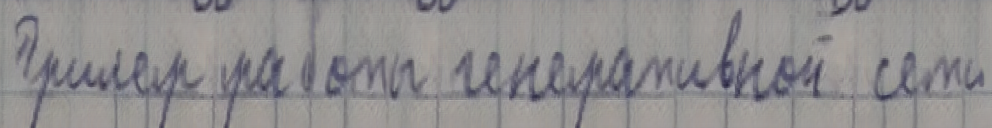
\includegraphics[width=0.9\textwidth]{img/gan_cyrillic}}
    \caption{Примеры результатов работы генеративно-состязательной сети ScrabbleGAN (сверху для набора HKR, снизу для набора Cyrillic Handwriting Dataset)}
    \label{fig:gan_example}
\end{figure}


\subsection{Проведение экспериментов}
\label{subsec:experiments}

Перед запуском экспериментов, рассмотрим результаты предложенных ранее методов для набора данных HKR~\cite{nurseitov2021handwritten}.
Более подробно эти методы описаны в секции~\ref{subsubsec:networks-russian}.
К сожалению, к настоящему моменту не было опубликовано результатов для набора Cyrillic Handwriting Dataset, предположительно в силу его недавнего появления.
Более подробное описание упомянутых наборов данных представлено в секции~\ref{subsec:datasets}.
Для оценки качества методов используются общепринятые стандартные метрики, описанные в секции~\ref{subsec:evaluation-metrics}.
Результаты работы существующих методов на наборе данных HKR представлены в таблице~\ref{tab:other_results}.

\begin{table}[h!]
    \centering
    \begin{tabular}{|p{2.5cm}|c|c|c|c|c|c|c|c|c|}
        \hline
        & \multicolumn{3}{c|}{HKR test1} & \multicolumn{3}{c|}{HKR test2} & \multicolumn{3}{c|}{HKR all} \\
        \cline{2-10}
        &  ACC  &  CER  &  WER  &  ACC  &  CER  &  WER  &  ACC  &  CER  &  WER  \\
        \hline
        \hline
        \cite{abdallah2020attention}          & -- & 4.13 & 18.91 & -- & 6.31 & 23.69 & -- & 4.5 & 19.02 \\
        \hline
        \cite{shonenkov2021stackmix} raw      & -- & -- & -- & -- & -- & -- & 71.1 & 3.49 & 22.5 \\
        \hline
        \cite{shonenkov2021stackmix} stackmix & -- & -- & -- & -- & -- & -- & 80.0 & 3.69 & 14.4 \\
        \hline
        \cite{shonenkov2021stackmix} best     & -- & -- & -- & -- & -- & -- & \textbf{82.0} & \textbf{3.49} & \textbf{13.0} \\
        \hline
    \end{tabular}

    \caption{Результаты на наборе HKR для существующих решений}
    \label{tab:other_results}
\end{table}

Следует уточнить, что показанные в таблице~\ref{tab:other_results} результаты получены не только благодаря удачному
выбору архитектуры модели распознавания и параметров обучения, но и из-за использования дополнительных техник
предобработки изображений (работа~\cite{abdallah2020attention}) и аугментации (работы~\cite{abdallah2020attention,shonenkov2021stackmix}).
Однако некоторые авторы делятся и промежуточными результатами, например, в работе~\cite{shonenkov2021stackmix} указаны <<сырые>> результаты модели (\textit{raw} в таблице),
а также результаты с отдельным использованием техники Stackmix (\textit{stackmix} в таблице).

Еще одна особенность, которую необходимо учитывать, связана с набором данных HKR, в котором предлагается тестировать модели на двух наборах:
\begin{itemize}
    \item первый тестовый набор \textit{test1} содержит почерки, присутствующие в тренировочном наборе, а слова -- новые;
    \item второй тестовый набор \textit{test2}, напротив, содержит слова, присутствующие в тренировочном наборе, но новые почерки.
\end{itemize}
Благодаря этому можно отследить, на чем именно переобучается модель -- на фиксированном словаре или стиле написания символов.
Как видно из таблицы~\ref{tab:other_results}, не все авторы публикуют значения метрик для каждого из тестовых наборов по отдельности,
что затрудняет подробный анализ их результатов.

В процессе проведения экспериментов предлагается сконцентрироваться именно на расширении набора данных,
т.е. добавлении в обучающий набор данных дополнительных новых изображений, созданных каким-либо способом.
Для этого предлагается анализировать изображения без проведения предобработки, так как она может потенциально привести к ухудшению качества изображений.
Помимо этого, необходимо зафиксировать аугментацию данных, т.е. набор искажений уже имеющихся данных без создания чего-либо нового.
Предлагается использовать с некоторой вероятностью следующие типы аугментации:
\begin{itemize}
    \item Адаптивное выравнивание гистограммы с ограниченным контрастом (CLAHE);
    \item Небольшие повороты изображения;
    \item Удаление небольших регионов изображения (Cutout);
    \item Искажение сетки (Grid Distortion);
    \item Размытие изображения;
    \item Сжатие JPEG.
\end{itemize}

В результате обзора различных архитектур моделей распознавания рукописного текста и из-за факта наличия открытого исходного
кода предлагаемых решений, для проведения экспериментов были выбраны следующие модели:
\begin{itemize}
    \item \textit{AttentionHTR}\footnote{\url{https://github.com/dmitrijsk/AttentionHTR}}~\cite{kass2022attentionhtr} --
    модель seq2seq~\cite{sutskever2014sequence} архитектуры, состоящая из сверточного модуля извлечения признаков ResNet~\cite{he2016deep},
    рекуррентного модуля разметки последовательности BiLSTM~\cite{hochreiter1997long} в качестве энкодера, и модуля внимания~\cite{bahdanau2014neural} в качестве декодера.
    В работе~\cite{kass2022attentionhtr} модель была обучена для текстов на английском языке и показала одни из лучших результатов на наборе данных IAM~\cite{marti2002iam}.
    \item \textit{Модель с архитектурой трансформер}\footnote{\url{https://github.com/t0efL/end2end-HKR-research}} --
    изначально обучалась на данных английского и русского языка, состоит из свёрточного модуля извлечения признаков ConvNext~\cite{liu2022convnet},
    трансформер-энкодера и двух декодеров: CTC~\cite{graves2006connectionist} и трансформер~\cite{vaswani2017attention}.
    Авторы модели не публиковали подробных результатов на конкретных наборах данных, однако архитектура модели интересна
    в силу того, что трансформеры являются многообещающим способом решения задачи.
\end{itemize}

Таким образом, выбрано две модели с различной архитектурой для проведения сравнительного анализа эффективности методов генерации дополнительного обучающего набора данных.
Для того, чтобы снизить эффект переобучения моделей, процесс обучения останавливается, если значение лосс-функции перестает уменьшаться 10 эпох подряд.
В силу ограниченности вычислительных ресурсов было решено ограничить обучение 100 эпохами, если предыдущий метод не остановил обучение ранее.

Так как для вышеперечисленных моделей были определены специальные методы стандартизации размера изображений, а также параметры обучения,
необходимые для получения наилучшего результато, было решено работать с ними без изменений.
Необходим лишь унифицированный метод загрузки изображений, использующихся при обучении моделей, для облегчения работы с разными моделями при одинаковых данных.
Кроме того, при обучении на нескольких наборах данных (в нашем случае это оригинальный и сгенерированный наборы) нужна
стратегия сбалансированного выбора изображений на каждой итерации обучения.
Предлагается на каждой итерации брать одинаковое количество данных из каждого набора,
предотвращая таким образом несбалансированность порядка обучающих данных.

\subsubsection{Генерация данных}

Для того, чтобы создать дополнительный набор данных для обучения, нужно выбрать текст для генерации изображений.
С этой целью было отобрано 300,000 слов и наборов слов из случайных статей, загруженных из Википедии\footnote{https://ru.wikipedia.org}.
Выбранные тексты были очищены от символов, не встречающихся в имеющихся наборах данных, а также были оставлены только уникальные элементы.
Для наборов данных HKR и Cyrillic Handwriting Dataset были выбраны различные корпусы текстов в силу того, что наборы символов в них сильно варьировались.
Общая статистика полученных корпусов слов показана на рисунках~\ref{fig:text_statistics_hkr} и ~\ref{fig:text_statistics_cyrillic}.

\begin{figure}[h!]
    \centering
    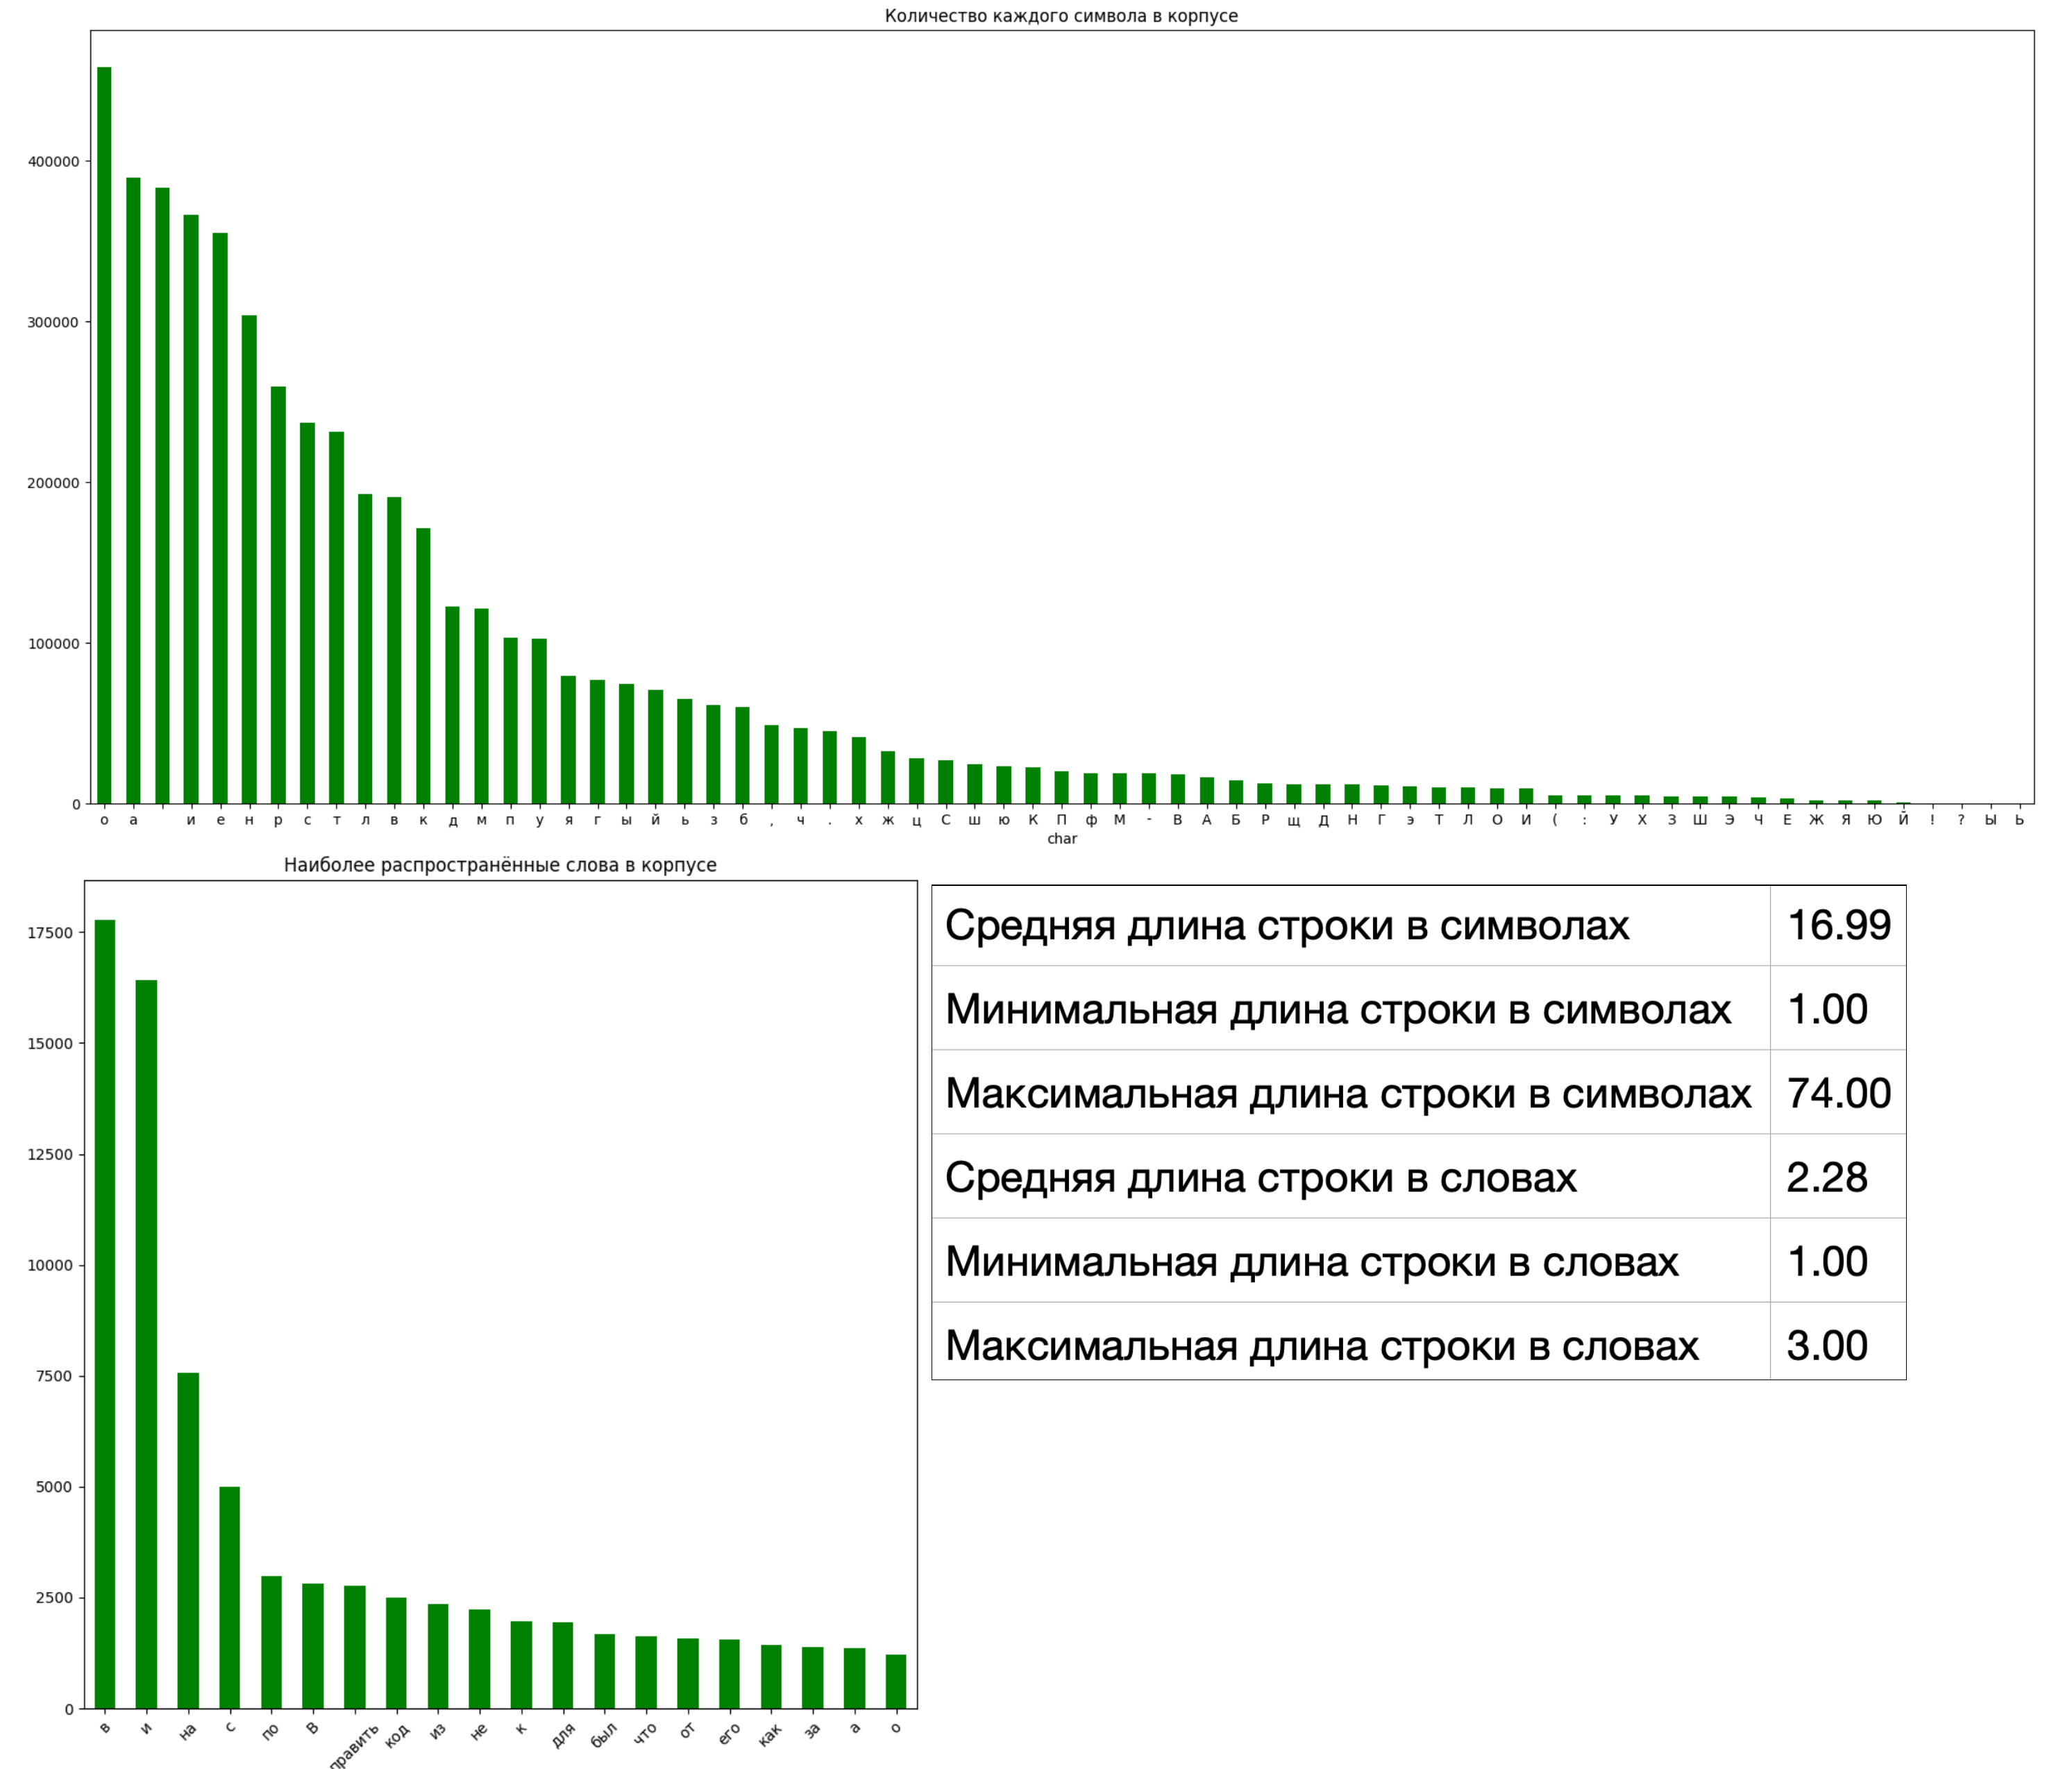
\includegraphics[width=\textwidth]{img/hkr_statistics}
    \caption{Общая статистика текстов, используемых при генерации изображений для набора HKR}
    \label{fig:text_statistics_hkr}
\end{figure}

\begin{figure}[h!]
    \centering
    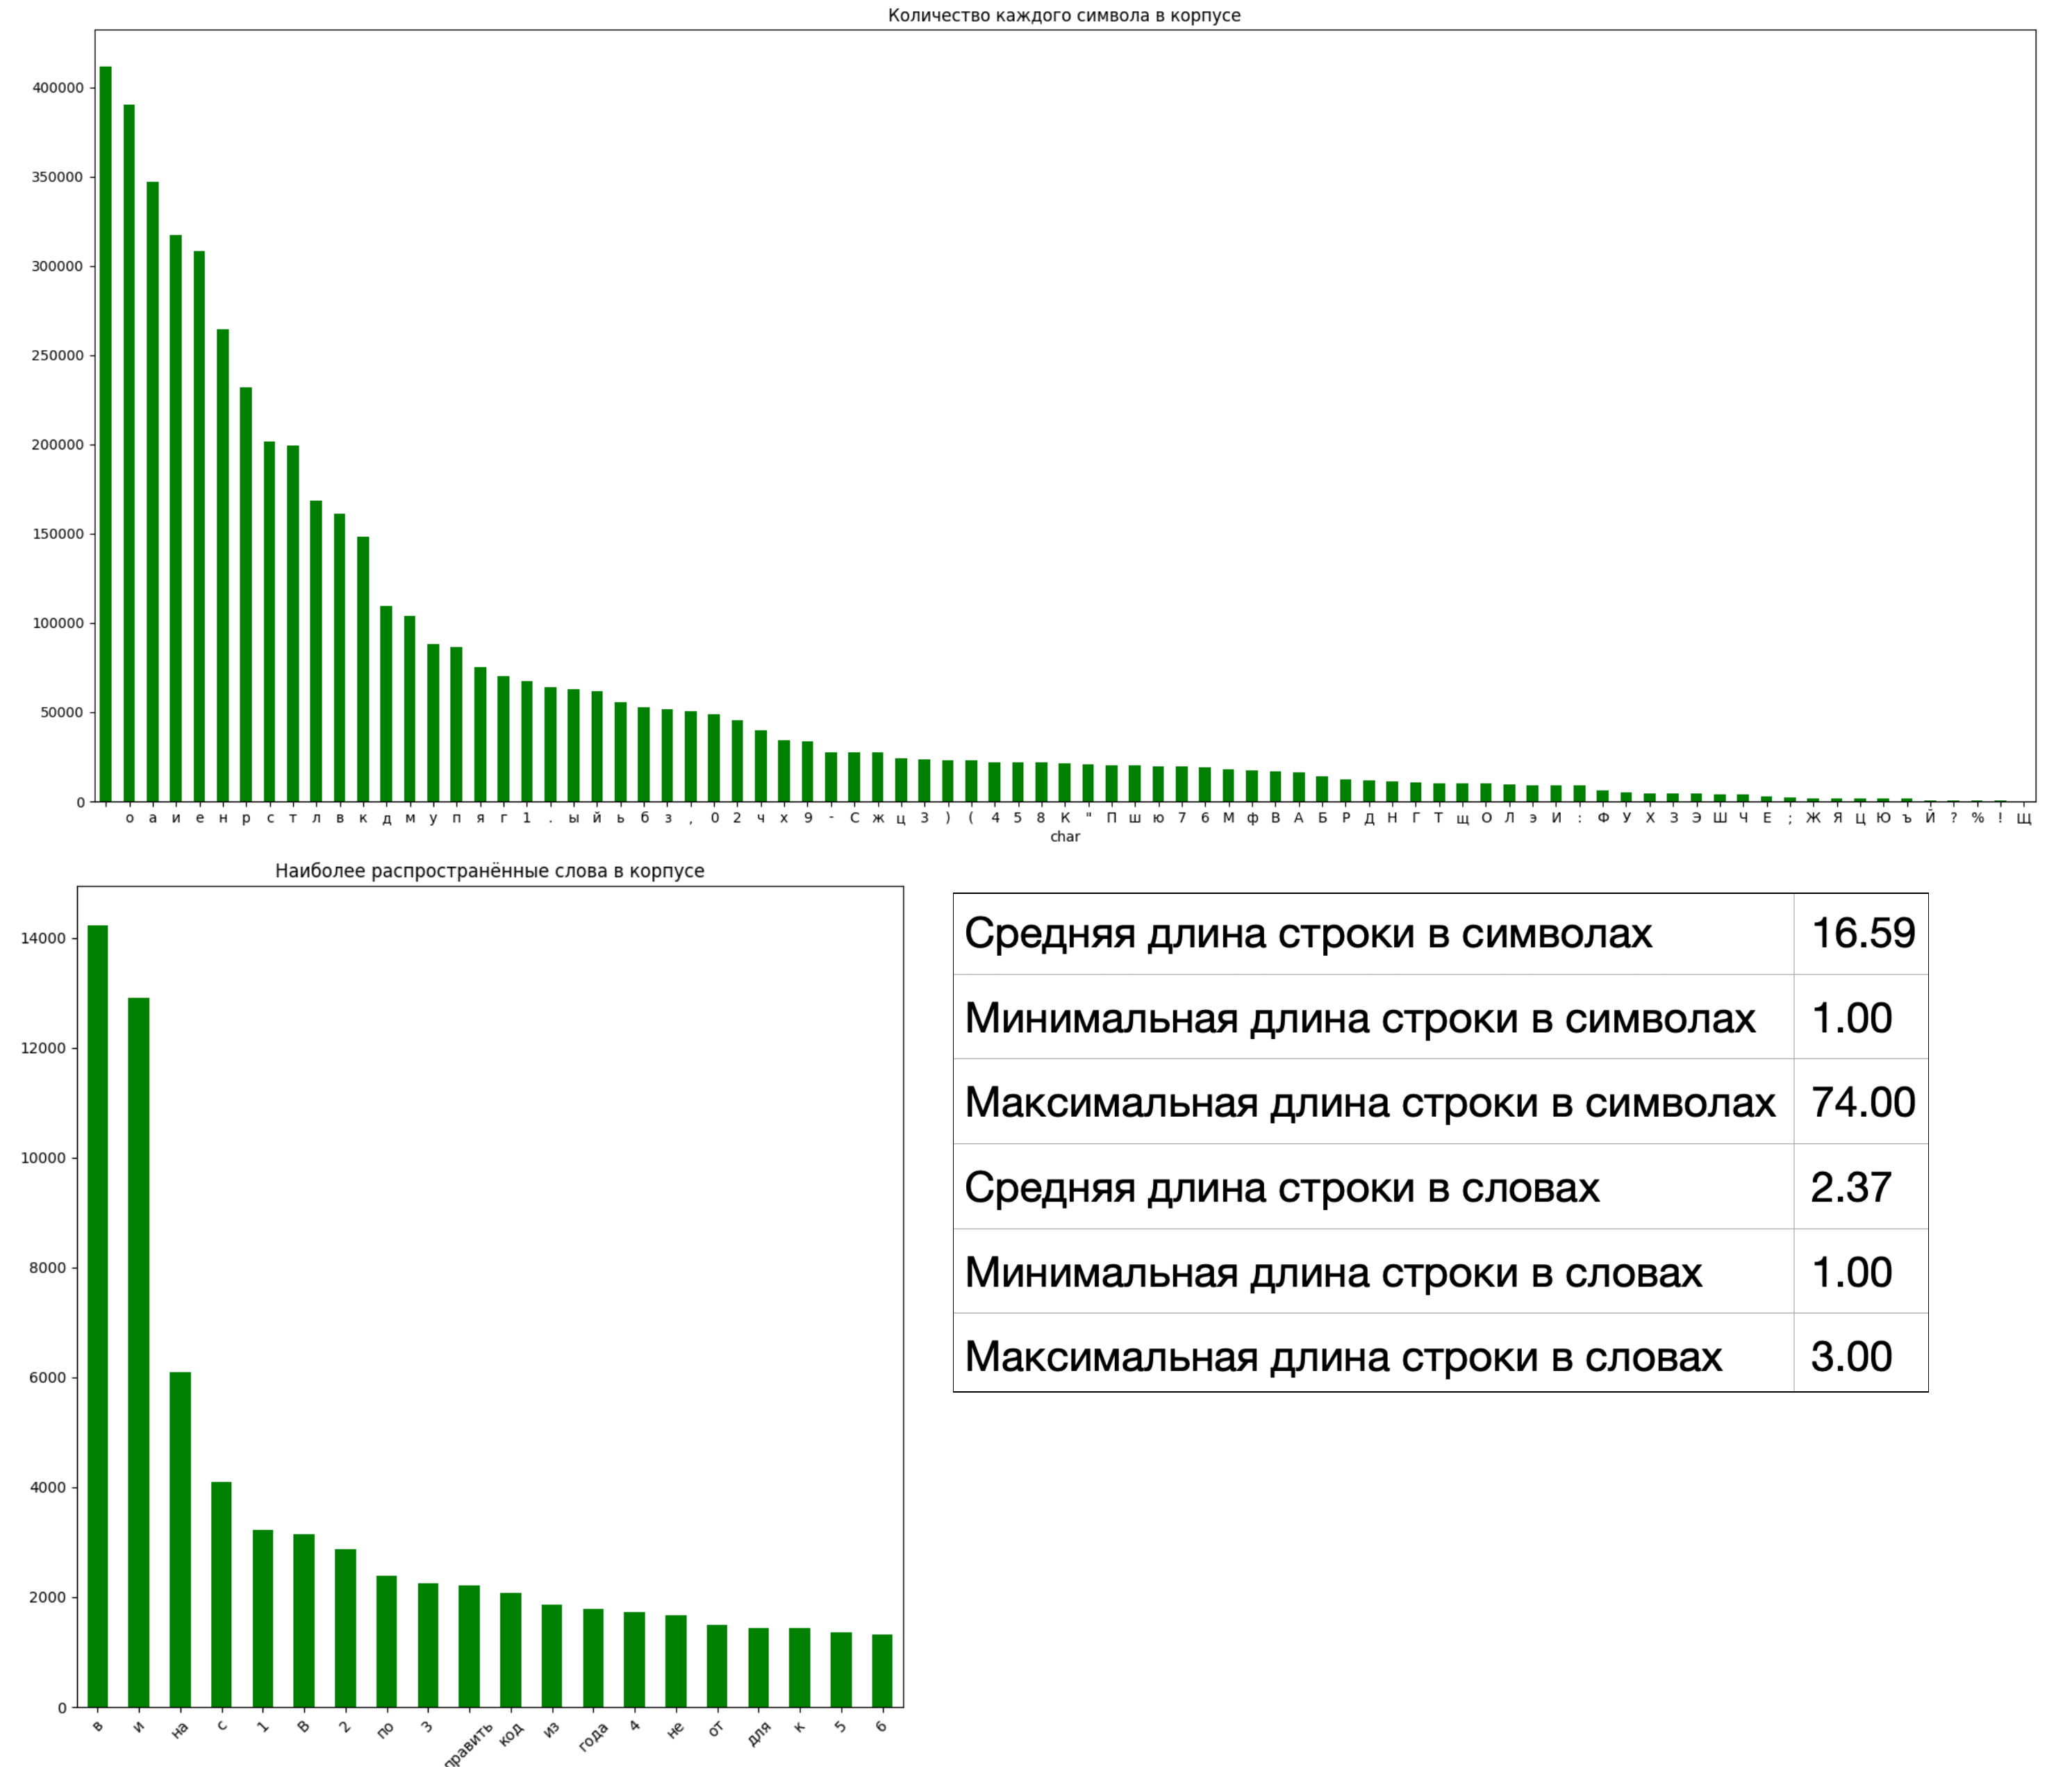
\includegraphics[width=\textwidth]{img/cyrillic_statistics}
    \caption{Общая статистика текстов, используемых при генерации изображений для набора Cyrillic Handwriting Dataset}
    \label{fig:text_statistics_cyrillic}
\end{figure}


Далее из полученных текстов генерировались их рукописные изображения следующими способами:
\begin{enumerate}
    \item \textit{С помощью рукописных шрифтов}:
    способ генерации изображений на основе шрифтов описан в секции~\ref{subsec:synthetic}.
    В результате поисков готовых шрифтов и создания новых с помощью базы символов было получено 65 различных рукописных шрифтов.
    Данные для наборов HKR и Cyrillic создавались похожим образом с отличием в количестве преобразований, применяемых к отрисованным изображениям.
    Для набора HKR не использовались преобразования, связанные с добавлением пятен на фон, так как изображения набора отличаются белым фоном без шумов.
    Для Cyrillic Handwriting Dataset использовались всевозможные преобразования, описанные в секции~\ref{subsec:synthetic},
    в силу большого стилевого разнообразия изображений, входящих в набор.
    \item \textit{С помощью метода Stackmix}:
    способ генерации c помощью Stackmix в описан в секции~\ref{subsec:stackmix}.
    Для этого на каждом из наборов HKR и Cyrillic была обучена нейронная сеть, предложенная авторами алгоритма,
    с рекомендуемыми ими параметрами обучения в течение 100 эпох.
    Далее данные были сгенерированы в соответствии с алгоритмом, указанным в секции~\ref{subsec:stackmix}.
    \item \textit{С помощью генеративно-состязательной сети ScrabbleGAN}:
    способ генерации изображений с помощью ScrabbleGAN описан в секции~\ref{subsec:gan}.
    На каждом наборе была обучена сеть ScrabbleGAN с параметрами, рекомендуемыми авторами исходного кода, в течение 100 эпох.
    После этого обученным моделям был переданы корпусы текстовых строк, для которых были сгенерированы синтетические
    данные, расширяющие наборы HKR и Cyrillic Handwriting Dataset.
\end{enumerate}

В результате генерации данных, на выходе получилось 6 различных дополнительных наборов, на которых можно обучать выбранные нейронные сети.
Важно отметить, что наборы данных состоят из одних и тех же слов, иначе результаты обучения невозможно интерпретировать.
Примеры изображений каждого из наборов представлены на рисунке~\ref{fig:generation_examples}.

\begin{figure}[h!]
    \centering
    \textbf{HKR}~~~~~~~~~~~~~~~~~~~~~~~~~~~~~~~~~~~~~~~~~~~~~\textbf{Cyrillic}\par\medskip
    \frame{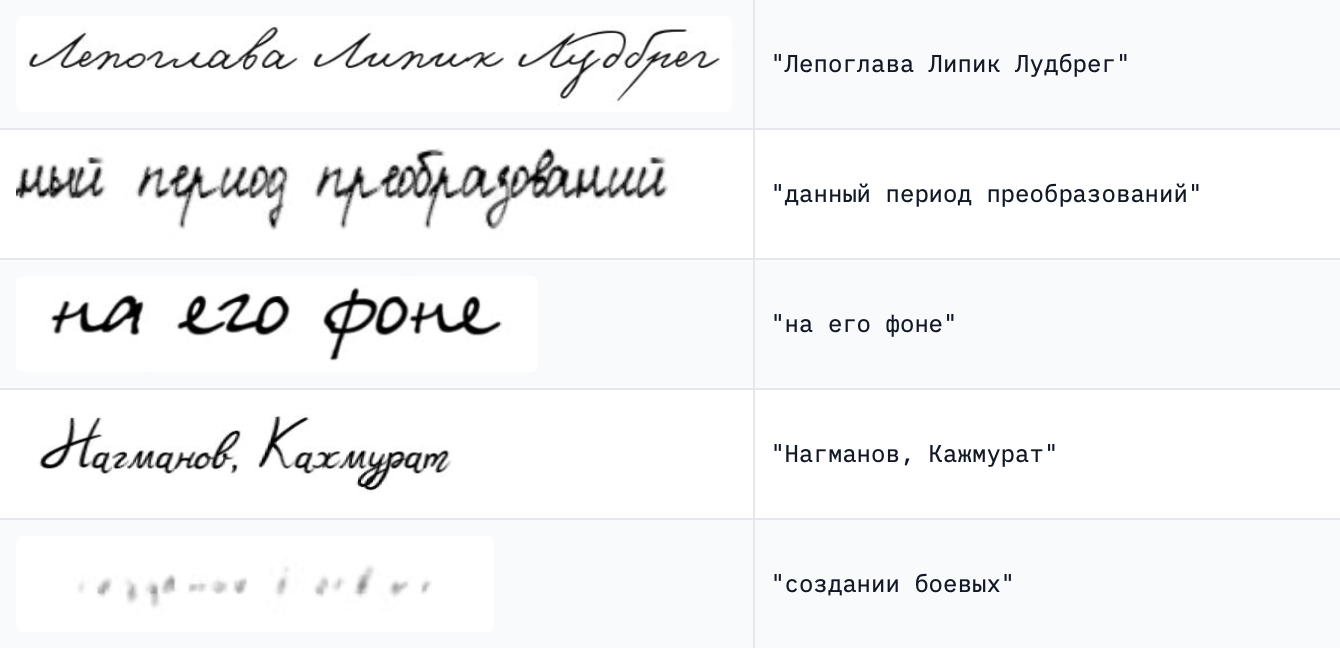
\includegraphics[width=0.47\textwidth]{img/huggingface_img/synthetic_hkr}}
    \frame{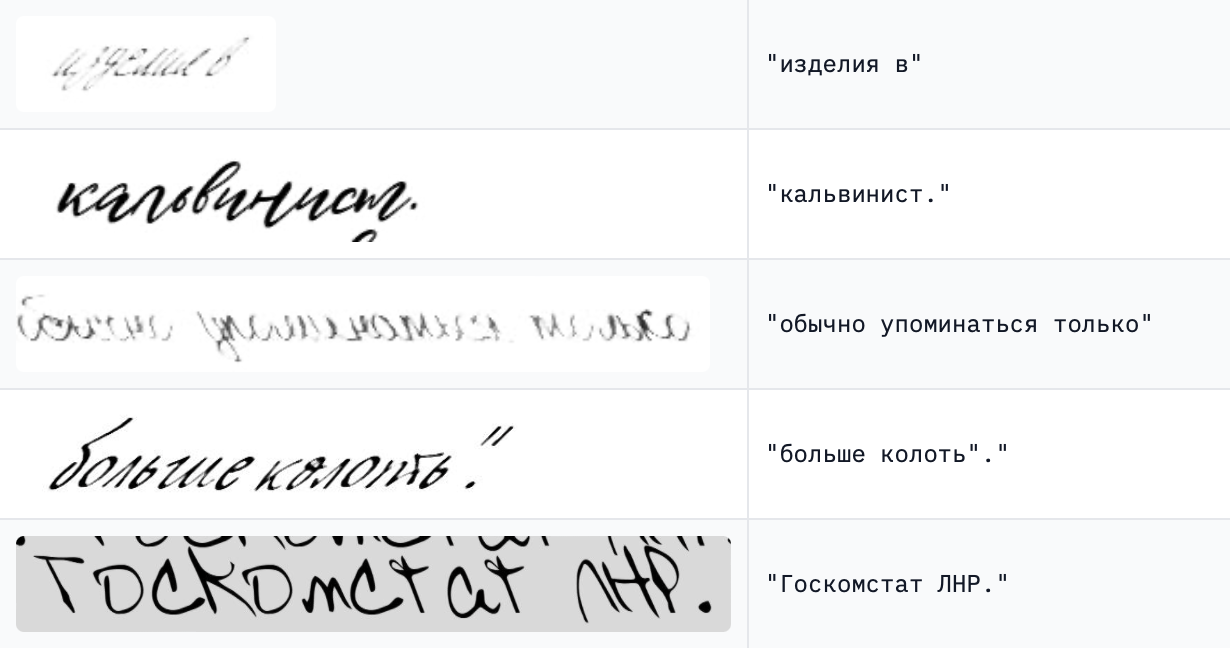
\includegraphics[width=0.43\textwidth]{img/huggingface_img/synthetic_cyrillic}}
    Генерация с помощью шрифтов\par\medskip
    \frame{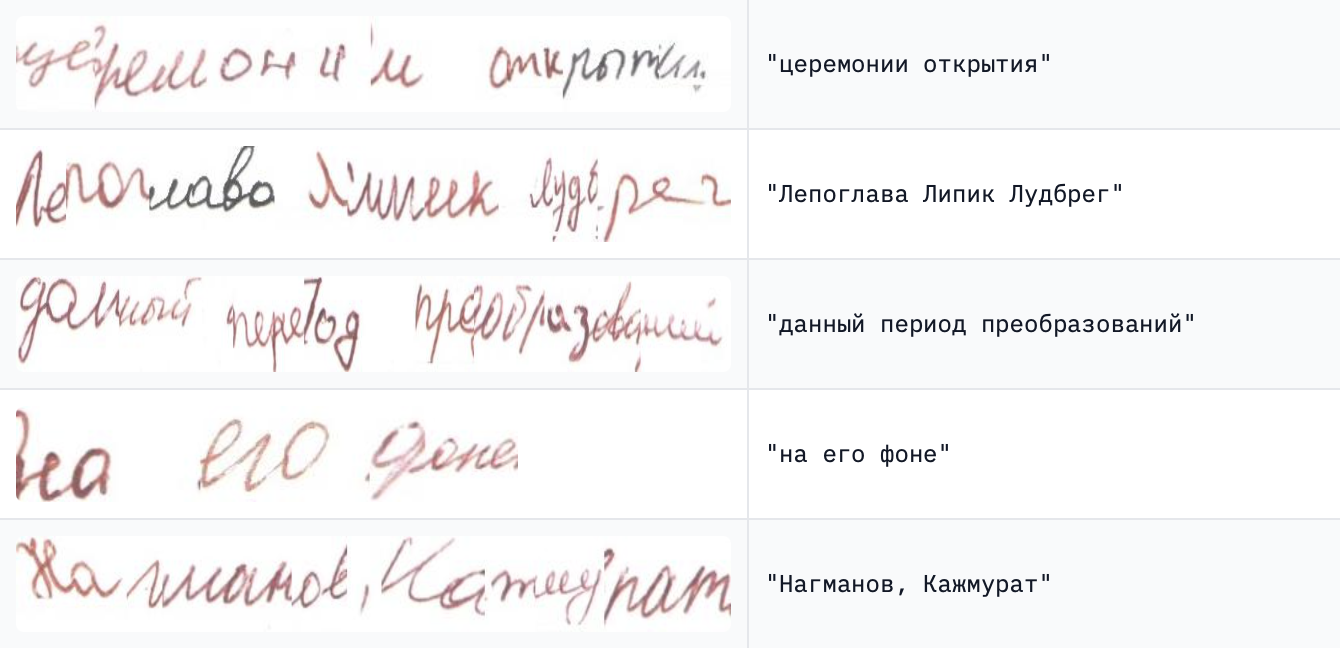
\includegraphics[width=0.47\textwidth]{img/huggingface_img/stackmix_hkr}}
    \frame{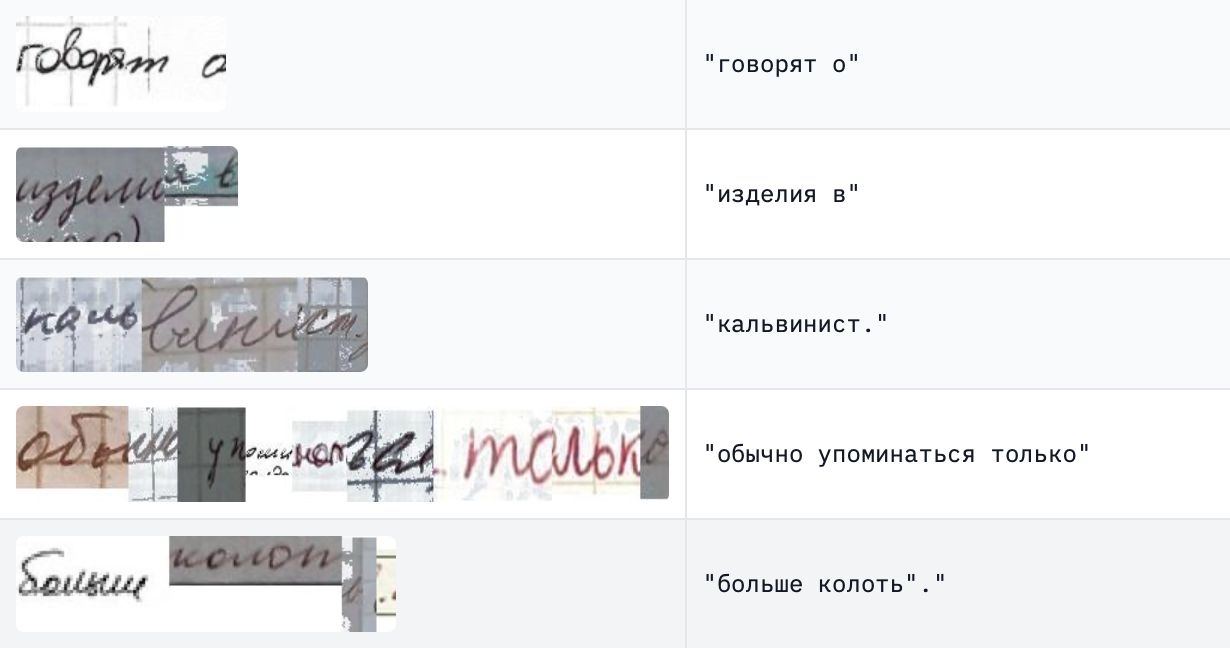
\includegraphics[width=0.43\textwidth]{img/huggingface_img/stackmix_cyrillic}}
    Генерация с помощью алгоритма Stackmix\par\medskip
    \frame{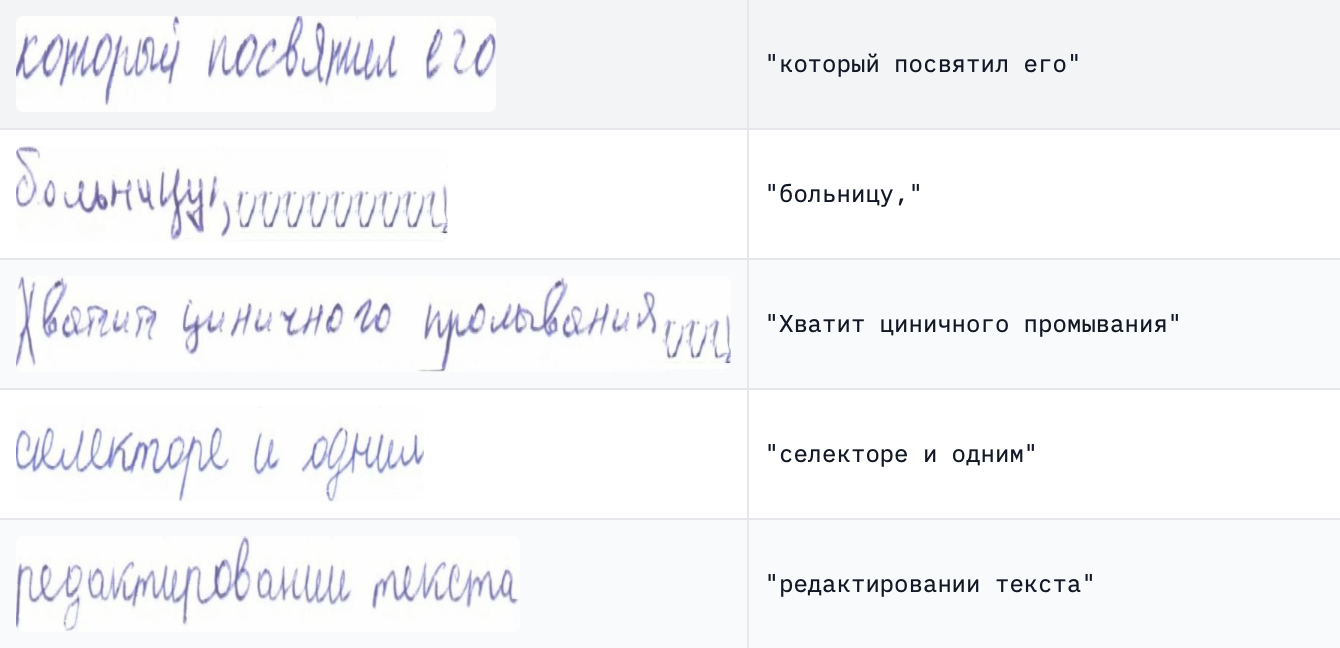
\includegraphics[width=0.47\textwidth]{img/huggingface_img/gan_hkr}}
    \frame{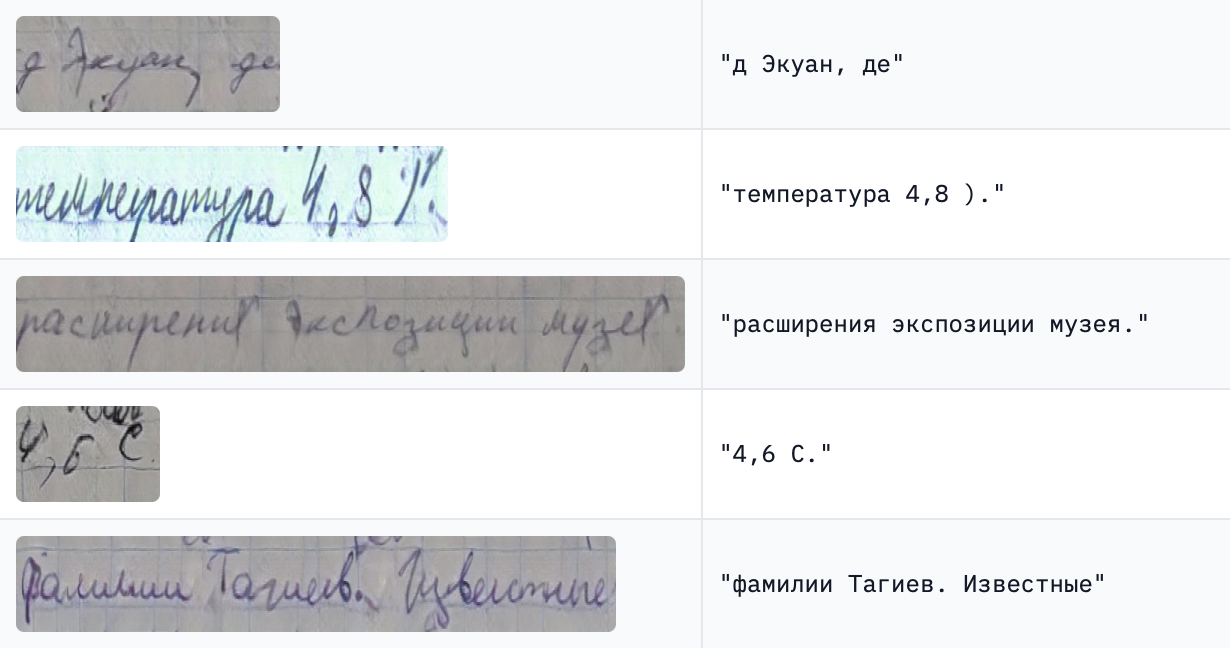
\includegraphics[width=0.43\textwidth]{img/huggingface_img/gan_cyrillic}}
    Генерация с помощью генеративно-состязательной сети ScrabbleGAN\par\medskip
    \caption{Примеры сгенерированных изображений из полученных наборов}
    \label{fig:generation_examples}
\end{figure}

Изображения примеров отражают некоторые описанные выше недостатки используемых методов генерации:
\begin{itemize}
    \item Относительное однообразие почерков и соединений символов в наборах, сгенерированных с помощью рукописных шрифтов.
    \item Нечитаемость некоторых слов на изображениях, созданных при помощи Stackmix из-за не всегда корректного нарезания
    слов на символы и несостыковок частей слов по высоте.
    Кроме того, в изображениях, созданных для набора Cyrillic Handwriting Dataset, видны существенные различия стилей фона и написания символов,
    которые склеиваются между собой, что вносит дополнительные сложности в распознавание изображенных слов даже человеком.
    \item Не всегда правильные соединения символов внутри слов в изображениях, сгенерированных сетью ScrabbleGAN.
    На изображениях некоторых слов сеть отрисовывает лишние артефакты, которые могут помешать при обучении модели распознавания.
    Также в некоторых изображениях, сгенерированных на основе набора Cyrillic Handwriting Dataset, встречаются сильные размытости, нечитаемый текст и
    разлиновка фона, подстраивающаяся под написанный текст.
\end{itemize}


\subsubsection{Анализ результатов}
\label{subsubsec:experiments_results}

\todo[inline]{Добавить информацию о лоссах}

В таблицах~\ref{tab:attention_htr_results},~\ref{tab:attention_htr_results_hkr},~\ref{tab:transformer_htr_results} и~\ref{tab:transformer_htr_results_hkr}
представлены результаты обучения нейронных сетей AttentionHTR и трансформера на наборах HKR и Cyrillic Handwriting Dataset
без использования дополнительных данных, а также с использованием наборов данных, сгенерированных тремя различными способами.
Дополнительные данные добавлялись на каждой итерации в процессе обучения в соотношении 50\% + 50\% для предотвращения дисбаланса в данных.
Качество распознавания каждой из обученных моделей оценивалось с помощью стандартных метрик accuracy, CER и WER, описанных в секции~\ref{subsec:evaluation-metrics}.
Результаты распознавания на наборе HKR показаны как для двух тестовых частей по отдельности, так и для всего тестового набора целиком.

\begin{table}[h!]
    \centering
    \begin{tabular}{|c|c|c|c|c|c|c|}
        \hline
              & \multicolumn{3}{c|}{HKR all} & \multicolumn{3}{c|}{Cyrillic} \\
        \cline{2-7}
                         &  ACC           &  CER           &  WER           &  ACC           &  CER           &  WER           \\
        \hline
        \hline
        Без генерации    & 63.67          & 22.55          & 37.64          & 37.95          & 18.53          & 60.63          \\
        Шрифты           & 64.69          & 13.55          & 31.78          & 49.09          & 13.12          & 49.23          \\
        Stackmix         & \textbf{68.96} &  \textbf{8.45} & \textbf{25.04} & \textbf{49.9}  & \textbf{12.44} & \textbf{46.03} \\
        GAN              & 64.69          & 12.09          & 30.28          & 37.69          & 16.68          & 59.1           \\
        \hline
    \end{tabular}
    \caption{Результаты обучения нейронной сети AttentionHTR}
    \label{tab:attention_htr_results}
\end{table}

\begin{table}[h!]
    \centering
    \begin{tabular}{|c|c|c|c|c|c|c|}
        \hline
        & \multicolumn{3}{c|}{HKR test1} & \multicolumn{3}{c|}{HKR test2} \\
        \cline{2-7}
                         &  ACC           &  CER           &  WER           &  ACC           &  CER           &  WER           \\
        \hline
        \hline
        Без генерации    & 39.12          & 42.1           & 67.41          & \textbf{87.86} & 3.31           & \textbf{8.33}  \\
        Шрифты           & 42.32          & 24.08          & 55.23          & 86.73          & \textbf{3.2}   & 8.69           \\
        Stackmix         & \textbf{53.08} & \textbf{13.64} & \textbf{40.13} & 84.61          & 3.34           & 10.2           \\
        GAN              & 43.11          & 21.08          & 51.65          & 85.96          & 3.24           & 9.24           \\
        \hline
    \end{tabular}
    \caption{Детальные результаты обучения AttentionHTR для набора HKR}
    \label{tab:attention_htr_results_hkr}
\end{table}

Исходя из значений метрик, показанных в таблицах~\ref{tab:attention_htr_results} и~\ref{tab:attention_htr_results_hkr},
можно сделать вывод, что лучшие результаты по части повышения качества обучения модели AttentionHTR показывает алгоритм Stackmix.
При этом, если рассматривать набор Cyrillic Handwriting Dataset, то можно заметить,
что результаты обучения на наборе, дополненном изображениями, сгенерированными с помощью шрифтов, не сильно хуже результатов для Stackmix.
В дополнение к этому, для набора HKR результаты расширения данных с помощью генеративно-состязательной сети ScrabbleGAN
практически аналогичны результатам расширения данных с помощью шрифтов, и способ на основе шрифтов явно выигрывает у ScrabbleGAN
на наборе Cyrillic Handwriting Dataset.
Из этих наблюдений можно сделать вывод о том, что метод генерации дополнительного синтетического набора данных с
помощью рукописных шрифтов не сильно уступает другим методам в плане повышения качества обучения моделей распознавания.
Однако этот метод имеет одно несомненное преимущество -- он не требует обучения тяжеловесных моделей и затачивания под конкретный набор данных.

В процессе анализа таблиц с результатами обучения моделей всплывает еще одна особенность, связанная с набором данных HKR.
Как было сказано ранее, тестовый набор HKR делится на две части, обладающие определенными особенностями,
которые оказывают сильное влияние на результаты, представленные в таблицах.
Тестовая часть \textit{test1} содержит новые слова и почеки, на которых модель обучалась, а часть \textit{test2}
содержит новые почерки, но старые слова, встречающиеся в тренировочной части набора.
По полученным значениям метрик можно сделать вывод о том, что модель AttentionHTR сильно переобучается на фиксированном наборе слов,
входящем в тренировочную часть набора HKR.
При этом влияние новых почерков на результаты распознавания минимально, если еще учитывать тот факт, что все изображения набора имеют похожий стиль.
Поэтому добавление дополнительных обучающих данных с новыми словами позволяет снизить эффект переобучения на фиксированном корпусе и
поднять значения метрик качества обученной модели.
Эффект переобучения на словах также может быть связан с тем, что набор данных HKR содержит большое количество изображений с одинаковым текстом:
при количестве элементов свыше 45 тысяч, уникальных текстовых единиц всего лишь 2808, некоторые из них незначительно отличаются друг от друга.
При этом валидационная часть набора состоит преимущественно из слов, содержащихся в тренировочной части (9133 слова из 9375).
Таким образом, обучение только на данных из тренировочной части набора HKR недостаточно оправданно, необходимы дополнительные данные с изображениями новых слов.


\begin{table}[h!]
    \centering
    \begin{tabular}{|c|c|c|c|c|c|c|}
        \hline
              & \multicolumn{3}{c|}{HKR} & \multicolumn{3}{c|}{Cyrillic} \\
        \cline{2-7}
                         &  ACC  &  CER  &  WER  &  ACC  &  CER  &  WER  \\
        \hline
        \hline
        Без генерации    & 66.68 & 10.56 & 29.08 & 48.57 & 11.71 & 44.87 \\
        Шрифты           &       &       &       &       &       &       \\
        Stackmix         &       &       &       & 59.00 & 8.35  & 37.27 \\
        GAN              & 72.18 & 7.49  & 23.51 &       &       &       \\
        \hline
    \end{tabular}
    \caption{Результаты обучения нейронной сети трансформер}
    \label{tab:transformer_htr_results}
\end{table}

\begin{table}[h!]
    \centering
    \begin{tabular}{|c|c|c|c|c|c|c|}
        \hline
        & \multicolumn{3}{c|}{HKR test1} & \multicolumn{3}{c|}{HKR test2} \\
        \cline{2-7}
                         &  ACC  &  CER  &  WER  &  ACC  &  CER  &  WER  \\
        \hline
        \hline
        Без генерации    & 45.08 & 19.24 & 53.33 & 87.96 & 2.02  & 5.22  \\
        Шрифты           &       &       &       &       &       &       \\
        Stackmix         &       &       &       &       &       &       \\
        GAN              & 53.00 & 13.05 & 41.68 & 91.07 & 2.03  & 5.62  \\
        \hline
    \end{tabular}
    \caption{Детальные результаты обучения трансформера для набора HKR}
    \label{tab:transformer_htr_results_hkr}
\end{table}


\subsection{Вывод}
\label{subsec:experiment_conclusion}

